\subsection{Overview}
\graphicspath{ {./texfiles/electrical/eimc/} }
%Electrical overview content here

\subsubsection*{Main requirements and design constraints}
Our high-voltage battery are required to 
\begin{itemize}
    \item power the EMRAX 188 MV motor, requiring a maximum of 120 A at 504 V for full power, through the traction inverter
    \item endure multiple runs 
    \item fit into the chassis appropriately
    \item do not exceed a weight limit of 30kg, also considering the efforts to remove it. Therefore, high energy (and power) density were important, removing the option of lead-acid batteries that are used in the railway sector. The high current ratings made specialized Lithium-Polymer cells one of the few, and the cheapest option available, which was to consider given the limited funds we had.
    \item be reliable and tested: The team designing the batteries originally come from a diverse background, having experience with manufacturing lithium battery packs. However, experimental innovative designs like supercapacitors or sodium ion cells were not feasible in the time. 
    \item be easily removable for maintenance
    \item be controlled by a battery management system, due to obvious safety reasons
    \item life cycle of at least 3 years for financial and environmental sustainability.
    \item have power headroom for future designs, being able to be reused. We therefore also ordered a surplus of 30 cells.
    \item cost less than 5000€, as a fund of a local bank is sponsoring us with 5000€ for the battery system (including BMS).
    \item charge at a rate of approximately 1C for time constraints.
    \item not heat up excessively, as we only opted for passive cooling.
\end{itemize}
The main design requirement was to satisfy the motor's needs, which are as follows:
\begin{figure}[H]
    \centering
    \includegraphics[width=0.9\textwidth]{texfiles/mech/eimg/propulsion/table_motor}
    \caption{Motor Specifications}
    \label{fig: Motor Specifications}
\end{figure}
The power ratings have been increased several times in the past two years, allowing for higher voltages. However, we stick to the initial data that we were given in the previous design. However the motor is tested at >800V DC maximum voltage. We will definitely not reach these levels.

\subsection{Electrical and mechanical design process}
%Electrical and mechanical design process content here
Our design followed these steps.
\begin{wrapfigure}{r}{0.25\textwidth}
    \centering
    \includegraphics[width=0.25\textwidth]{texfiles/elec/eimg/BatteryDesignProcess}
    \caption{Heuristic for Finding Battery Parameter}
\end{wrapfigure}
For easier simulations, we used a matlab script with different parameters, which is publicly accessible via Github \footnote{\href{https://github.com/Team-Tachyon-e-V/battery_model}{Link to our battery model estimation}}:
\subsubsection*{Pod Characteristics} 
Some constant mechanical coefficients for the pod's movement that we assumed in our calculations:

\begin{align*}
m_{\text{fzg}} &= 250 \, \text{kg} & \text{(Vehicle Mass)} \\
m_{\text{zul}} &= 50 \, \text{kg} & \text{(Payload)} \\
c_L &= 0.8 & \text{(Drag Coefficient)} \\
\rho_L &= 1.2 \, \text{kg/m}^3 & \text{(Air Density)} \\
f_r &= 0.02 & \text{(Kinetic Friction Coefficient)} \\
g &= 9.81 \, \text{m/s}^2 & \text{(Gravitational Acceleration)} \\
A &= 1.5 \times 0.3 \, \text{m}^2 & \text{(Frontal Area)} \\
e_{i1} &= 1.2 & \text{(Mass Factor for Rotating Part)} \\
\text{Gradient} &= 5\% & \text{(Inclination Gradient Percentage)} \\
\alpha &= \arctan\left(\frac{\text{Gradient}}{100}\right) & \text{(Inclination Gradient Angle)}
\end{align*}

\subsubsection*{Mass Calculation}

Effective mass that will be accelerated:

\begin{align*}
m_{\text{acc}} =  e_{i1} \times m_{\text{fzg}} + m_{\text{zul}} = 1.2 \times 300 \, \text{kg} = 360 \, \text{kg}
\end{align*}

\subsubsection*{Vehicle Dynamics Parameters}

Parameters related to the pod's movement:

\begin{align*}
v_{\text{init}} &= 0 \, \text{m/s} & \text{(Starting Velocity)} \\
v_{\text{max}} &= \frac{60}{3.6} \, \text{m/s} \approx 16.67 \, \text{m/s} & \text{(Maximum Velocity)} \\
s_f &= 150 \, \text{m} & \text{(Pod Distance)} \\
R_d &= 0.1 \, \text{m} & \text{(Radius of Driving Wheel)} %should be diameter
\end{align*}

\subsubsection*{Motor Parameters}

Motor's specifications:

\begin{align*}
P_{\text{peak}} &= 37 \times 1000 \, \text{W} & \text{(Power at 7000 rpm)} \\
\text{eff} &= 0.96 & \text{(Efficiency)} \\
P_{\text{motor}} &= 0.96 \times 37000 \, \text{W} = 35520 \, \text{W}
\end{align*}

\subsubsection*{Resistance Calculation for Continuous Power}

We add all resistive forces against the pod's motion, taking into account that we drive in a non-vacuum environment:

\begin{align*}
F_{\text{roll}} &= 0.02 \times 300 \times 9.81 \times \cos\left(\arctan\left(\frac{5}{100}\right)\right) \\
F_{\text{luft}} &= 0.5 \times 0.8 \times 1.2 \times (1.5 \times 0.3) \times (16.67^2) \\
F_{\text{st}} &= 300 \times 9.81 \times \sin\left(\arctan\left(\frac{5}{100}\right)\right)
\end{align*}

\subsubsection*{Maximum Acceleration Calculation}

Pod's maximum acceleration:

\begin{align*}
a_{\text{max}} = \frac{\left(\frac{35520}{16.67}\right) - F_{\text{roll}} - F_{\text{luft}} - F_{\text{st}}}{360}
\end{align*}

\subsubsection*{S-Curve Generation}

Timing for acceleration and deceleration phases:

\begin{align*}
T &= \left(\frac{a_{\text{max}}}{j_{\text{max}}}\right) + \left(\frac{16.67}{a_{\text{max}}}\right) + \left(\frac{150}{16.67}\right)
\end{align*}

\subsubsection*{Energy Demand}

Energy demand for the journey: \text{energy\_bed\_wh} = \text{Energy demand in Wh}

\subsubsection*{Battery Parameters}
%% Voltage and Current Need(from data sheet)

\begin{align*}
V_{\text{bed}} &= 490 \, \text{V}; \\
I_{\text{bed}} &= 100 \, \text{A}; \\
%% Battery Parameters
U_{\text{zell}} &= 4.2 \, \text{V}; \\
C_{\text{zell\_ah}} &= 6.1 \, \text{Ah}; \\
C_{\text{rate}} &= 35; \\
\text{SoC\_max} &= 80\%; \\
\text{SoC\_min} &= 40\%; \\
\textbf{Required battery configuration:}; \\
n_{\text{ser}} &= \left\lceil \frac{V_{\text{bed}}}{U_{\text{zell}}} \right\rceil; \\
C_{\text{tot}} &= \frac{\text{energy\_bed\_wh}}{n_{\text{ser}} \times U_{\text{zell}} \times \text{eff\_mech}}; \\
n_{\text{par}} &= \left\lceil \frac{C_{\text{tot}}}{C_{\text{zell\_ah}} \times \left(\frac{\text{SoC\_max} - \text{SoC\_min}}{100}\right)} \right\rceil; % Add semicolon at the end
\end{align*}
The S-curves are simple, as follows:
\begin{figure}[h]
    \centering
    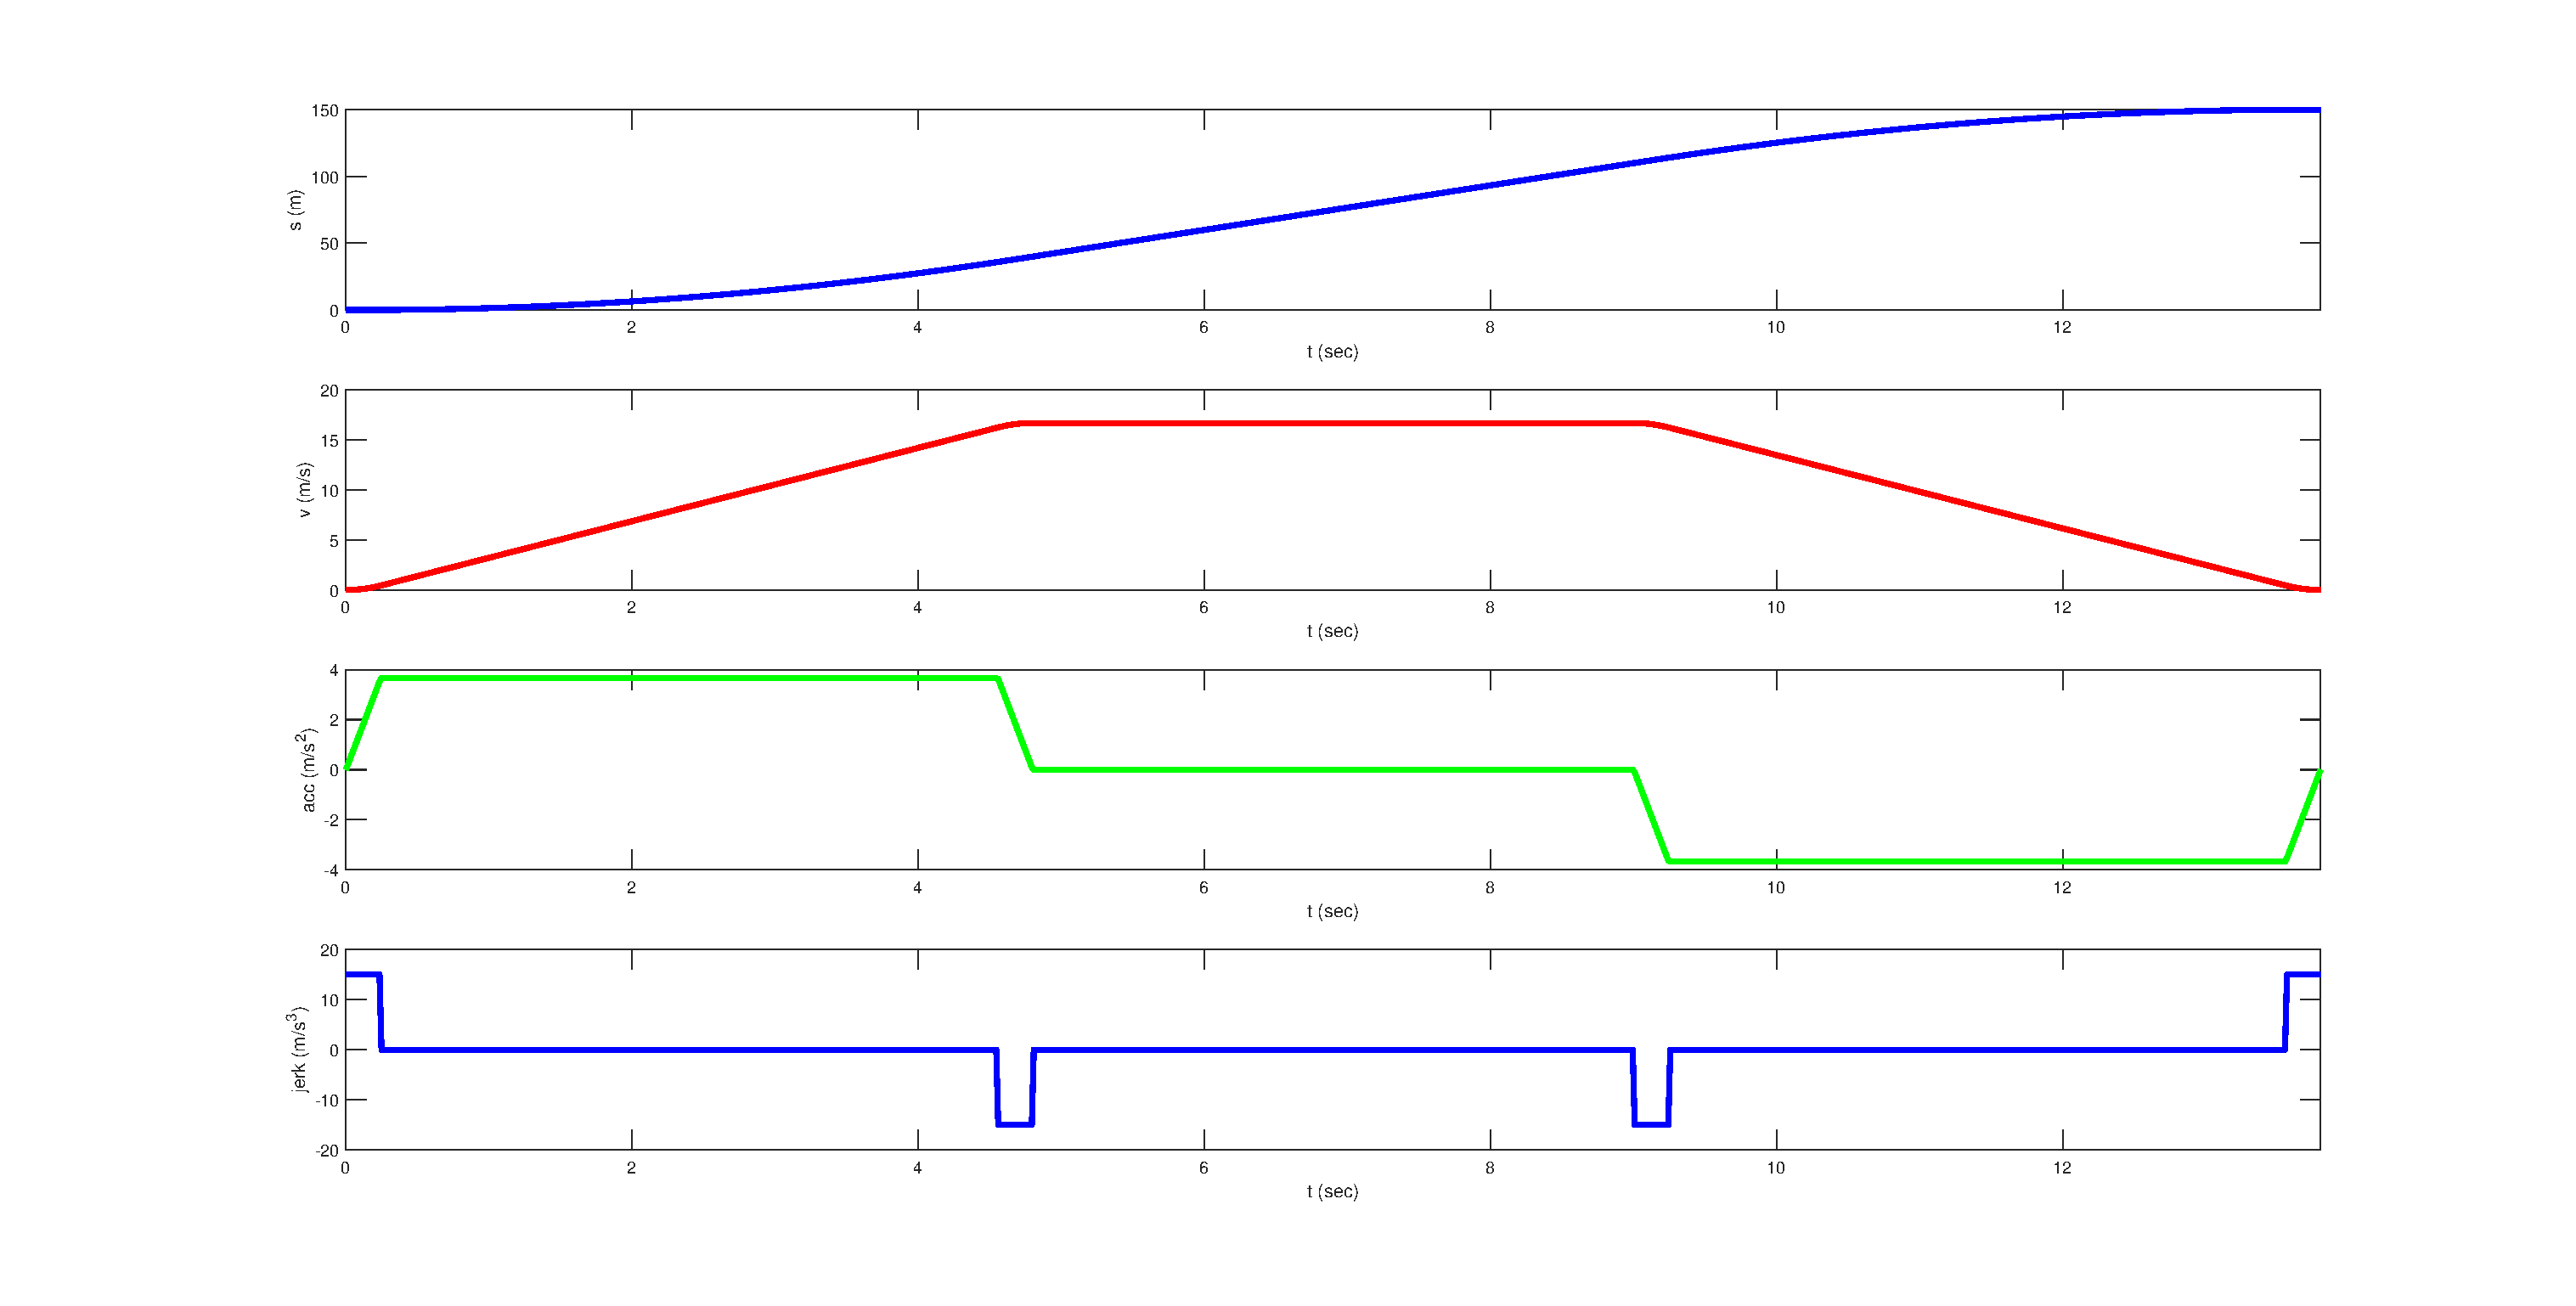
\includegraphics[width=0.9\textwidth]{texfiles/elec/eimg/battery_run_model}
    \caption{Run model}
    \label{img: runmodel}
\end{figure}
The results showed that we needed 117 x 1 cells in series, which can be explained because we assumed to be able to use the maximum voltage, not the nominal voltage of the battery cells. We are able to run 27.47 runs, even with keeping our state of charge between 40 and 80 percent, saving battery health \footnote{We follow general advice that the optimal SOC lay between 0.2 to 0.8, and exceeding this range is not per se damaging to the battery, but shortening its life span, which we try to avoid}.
\subsubsection{Schematics and drawings.}
The CAD models of the battery pack are shown in the following. We visually cut the box open to show the inside structure. For the environment, please refer to the \hyperref{sec:chassis}{Chassis section}. \\

\begin{figure}[h]
    \centering
    \includegraphics[width=0.9\textwidth]{texfiles/elec/eimg/BatteryCell}
    \caption{Battery cell}
    \label{img: Batterycell}
\end{figure}
\begin{figure}[h]
    \centering
    \includegraphics[width=0.9\textwidth]{texfiles/elec/eimg/BatteryAssemblyDiag}
    \caption{Battery pack}
    \label{img: Batterypack}
\end{figure}
\begin{figure}[h]
    \centering
    \includegraphics[width=0.9\textwidth]{texfiles/elec/eimg/BatteryAssemblySide}
    \caption{Battery pack from the top}
    \label{img: Battery pack from the side}
\end{figure}
\begin{figure}[h]
    \centering
    \includegraphics[width=0.9\textwidth]{texfiles/elec/eimg/BatteryAssemblyTop}
    \caption{Battery pack from the top}
    \label{img: Battery pack from the top}
\end{figure}
\subsubsection{Temperature simulations for vacuum conditions.}
For our heat simulations, we used the software of ANSYS. By vacuum conditions, we assumed the
lack of gas flow, which eliminates the cooling heat flow from winds. The simulation tool solves
the heat transfer equation \( \frac{\partial T}{\partial t} = \alpha \left( \frac{\partial^2 T}{\partial x^2} + \frac{\partial^2 T}{\partial y^2} + \frac{\partial^2 T}{\partial z^2} \right) \)
by discretizing through Finite-Element-Methods.
\subsection{Electrical system characteristics}
%Content of the electrical system characteristics here
\subsection{Interface with other system}
%Interface with other system content here n
\subsubsection{Control systems of the boards}
We configure the BMS prior to the competition, and do not plan to change any settings during the competition. It sends telemetry data over CAN. \\
All the electric subsystems are located within the pod. \\

The physical connection matrix is as following:
\begin{table}
    \centering
    \begin{adjustbox}{width=\textwidth,center}
    \begin{tabular}{|c|c|c|c|c|c|c|}
    \hline
    From | To & \text{LV Battery} & \text{HV Battery} & \text{BMS} & \text{Traction Inverter} & \text{Motor} & \text{Cooling System} \\
    \hline
    \text{LV Battery} & - & - & Powers & \text{Powers control system} & - & \text{Powers pump and control system} \\
    \hline
    \text{HV Battery} & - & - & Connects to & \text{Provides power} & - & - \\
    \hline
    \text{BMS} & - & - & \text{Controls} & - & - & - \\
    \text{Traction Inverter} & - & - & - & - & \text{Propels} & X \\
    \hline
    \text{Motor} & - & - & - & - & - & - \\
    \hline
    \text{Cooling System} & - & - & - & \text{Cooling} & \text{Cooling} & \text{Cooling (implicitly)} \\
    \hline
    \end{tabular}
\end{adjustbox}
\caption{Physical connection matrix}
\label{Physical connection matrix Battery}
\end{table}

The data connection matrix is as following. All communication between boards are via CAN, if not specified otherwise:

\begin{table}
    \centering
    \begin{adjustbox}{width=\textwidth,center}
    \begin{tabular}{|l|c|c|c|c|c|c|c|c|}
    \hline
    From $\backslash$ To & LV Battery & HV Battery & BMS & Traction Inverter & Motor & Cooling System & Brakes Controller & Telemetry Unit  \\
    \hline
    LV Battery & - & - & - & - & - & - & - & - \\
    HV Battery  & - & - & Discharge rate, voltage level & - & - & - & - & - \\
    BMS & controls & controls & - & - & - & - & - & sends data \\
    Traction Inverter & - & - & - & - & - & - & - & sends data \\
    Motor & - & - & - & - & - & - & - & - \\
    Cooling System & - & - & - & - & - & - & - & sends data \\
    Brakes Controller & - & - & - & - & - & - & - & sends data \\
    Telemetry Unit & - & - & updates limits & sends commands & - & sends target rates & sends commands & - \\
    \hline
    \end{tabular}
    \end{adjustbox}
    \caption{Data connection matrix}
    \label{data-connectivity-matrix-battery}
\end{table}


\subsection{Final system description}
%Description of the system here
\subsubsection{Battery Cells}

High Voltage Network: \\
Our high voltage battery will make use of lithium-ion polymer technology. We use 120 pouch-format cells from Shenzhen GrePow Battery Co. Ltd rated at 45C maximum discharge that we plan to connect in series. 
The finished package (main battery pack) will be assembled by the team, helped by the ISEA institute of RWTH Aachen University.
We are going to connect the 120 cells connected in series and that will have 1 parallel line. This will roughly have 504 Volt at max (using \(120 * 4.2V = 504 V \) ) 
which provides sufficient electricity to power the motor.
The battery pack will provide up to ~350 Amps of DC current available to the inverter. However, neither the inverter nor the motor is not rated for such high currents nominally, and we are not trying to use the full power of the battery pack.
\newline
Therefore, the maximum output current of the HV Battery will be rated at 120 A maximum (peak) and 74 A continuous. As the peak duration is at 120s, and our runs are at most 10s, we will set the limit of the inverter to 120A for the competition.
\subsubsection{BMS}
Our centralized battery management system, the Orion BMS 2, connected to the HV battery, protects it and improves its health and efficiency.
It is an OEM product. \\
It acts by: \begin{itemize}
    \item Monitors every cell voltage in series
    \item Intelligent cell balancing (efficient passive
    balancing)
    \item Enforces min. and max. cell voltages
    \item Enforces maximum current limits
    \item Enforces temperature limits
    \item Monitors state-of-charge and pack health, internal resistance
    \item Controls discharging and charging
    \item Retains lifetime data about battery history
\end{itemize}

The Orion BMS 2 facilitates real-time monitoring and management of each cell within the HV battery pack, 
which consists of 120 lithium-ion polymer cells arranged in a series configuration to achieve a nominal voltage of 504V. 
This arrangement necessitates precise control and monitoring to prevent overcharging, deep discharging, and to ensure balanced 
cell voltages, all of which are within the Orion BMS 2's capabilities.

1. **Cell Voltage Monitoring and Balancing:** The BMS continuously monitors the voltage of each cell, ensuring 
that all cells operate within their safe voltage range. Cell balancing is performed to equalize the charge across all cells,
thereby enhancing the battery pack's overall efficiency and lifespan.

2. **Temperature Monitoring:** 
Given the high energy density of the HV battery pack, 
thermal management is paramount. The Orion BMS 2 monitors the temperature of individual cells 
and the battery pack as a whole, activating cooling measures when necessary and preventing operation 
under extreme temperatures that could damage the battery or compromise safety.
The Orion BMS 2 itself tracks the temperature of 8 individual cells. 28 other cells are measured by the Thermal Controller.

3. **State of Charge (SoC) and State of Health (SoH) Estimation:** 
SoC and SoH estimations are important for optimal battery utilization and health maintenance. 
The Orion BMS 2 employs advanced algorithms to provide these estimates, 
ensuring that the battery's capacity is used efficiently.


The integration of the Orion BMS 2 encompasses several safety mechanisms designed to protect the battery pack, the hyperloop pod, and its occupants:

1. **Overcurrent and Short Circuit Protection:** By monitoring the current flowing in and out of the battery pack, the Orion BMS 2 can detect overcurrent conditions and short circuits, initiating immediate shutdown procedures to prevent damage and ensure safety.

2. **High and Low Voltage Protection:** The BMS prevents the battery from exceeding its maximum voltage during charging and dropping below its minimum voltage during discharge, thereby avoiding scenarios that could lead to reduced battery life or safety hazards.

3. **Thermal Runaway Prevention:** Through its temperature monitoring capabilities, the Orion BMS 2 can detect the onset of thermal runaway—a dangerous condition where one cell's failure can lead to a cascading failure of adjacent cells—and take corrective actions to isolate the problem and mitigate potential damage.

Efficiency Enhancements

By optimizing the operational parameters of the HV battery pack, the Orion BMS 2 contributes significantly to the efficiency and performance of the hyperloop prototype:

1. **Energy Optimization:** By ensuring that all cells are balanced and operate within their optimal voltage and temperature ranges, the BMS maximizes the energy extracted from the battery pack, contributing to the hyperloop's range and speed capabilities.

2. **Lifecycle Extension:** Through diligent monitoring and management, the Orion BMS 2 extends the useful life of the HV battery pack, reducing the environmental impact and operational costs associated with battery replacement.

3. **Predictive Maintenance:** By providing detailed data on the SoC and SoH, the Orion BMS 2 enables predictive maintenance, allowing for timely interventions that prevent unscheduled downtimes and extend the battery's lifespan.

Conclusion

The integration of the Orion BMS 2 with the HV battery pack in our hyperloop prototype represents a critical step towards ensuring the system's safety, efficiency, and reliability. Through its comprehensive monitoring and management capabilities, the Orion BMS 2 ensures that the HV battery pack operates within its optimal parameters, significantly contributing to the prototype's overall performance and safety profile. As we progress towards the final stages of the FDD, the detailed exploration of the Orion BMS 2's functionalities underscores our commitment to leveraging advanced technologies for the enhancement of hyperloop transportation systems.
\subsubsection{Insulation Monitoring Device}
The Insulation Monitoring Device that is mandatory for EHW participants, as well as Formula Students teams, is not built inhouse, after receiving the respective advice from the EHW technical jury. By reaching out to Bender, we received their device through their Formula Students policy. It is configured for ...


\subsection{Manufacturing process}
%Manufacturing process content here
Our PCB Design

\subsubsection{PCBs}
Prototyping: Prototype PCBs are fabricated in the FabLab associated with our university. The FabLab provides access to PCB manufacturing equipment and materials, enabling the rapid production of prototypes for initial testing and design validation. Once the PCBs are fabricated, they are assembled manually by our team members. Bigger PCBs are assembled in the facilities of the FabLab with the manual Pick and Place Machine and a reflow oven.

Production: We ordered our final PCBs from JLCPCB, a leading PCB manufacturing service. In addition to JLCPCB, we also collaborate with Würth Elektronik who produce PCBs in Germany, aligning with our goal of sustainability.

\subsubsection{Batteries}
Our phases of production followed this structure:
\begin{figure}[H]
    \centering
    \includegraphics[width=0.9\textwidth]{texfiles/elec/eimg/BatteryProduction}
    \caption{Stages of Production of Battery Pack}
    \label{img: batteryproduction}
\end{figure}

We produced the battery packs in cooperation with the ISEA (Institute for Power Electronics and Electrical Drives) at RWTH, whose experience helped us to assemble and design the parts more efficiently and more safely, as we had a considerable high voltage system.

The casing will consist of polycarbonate. Polycarbonate is a material that is durable, lightweight, and impact resistant. The problems with material degradation through UV emissions do not impact us substantially, as we cover the battery pack inside the shell for most of the time. We will have safety measures preventing too much exposure to UV radiation. Also, the degradation is mainly of cosmetic nature (https://link.springer.com/article/10.1007/s11668-020-01002-9).

\subsubsection{Material Selection:}
Battery Case: It will be made of flame-retardant grades of ABS (Acrylonitrile Butadiene Styrene) because of its lightweight, impact-resistant, and easy molding into complex shapes.

Vibration Protection Material: Neoprene foam will be used to protect against vibration because of its durability and resilience. It provides effective vibration damping and is resistant to oils, chemicals, and temperature variations.

Cell Holder: Polypropylene (PP) will be used for pouch cell holders due to its lightweight, chemical resistance, and ease of molding. It provides good structural support and can be designed with features such as tabs or grooves to securely hold the cells in place.

Thermal Interface Material: We are going to use aluminum foil to increase the heat flow of the cells.

Compression Protection Element: We will use Silicone Rubber due to its flexibility, durability, and resistance to heat and chemicals. It will provide cushioning against mechanical shocks and vibrations while securely holding the cells in place.

Busbar: Busbar will be made of pure copper as it needs to transfer a high rate of discharge due to its low resistance.

Thermal Protection Material: As we are depending on passive cooling of the battery, we will not use any thermal protection material to ensure the air passing through the cells maintains the operating temperature.

Fire Retardant Material: A plate will be placed over the connections made of flame-retardant grades of ABS (Acrylonitrile Butadiene Styrene) to ensure the slow propagation of flame.

Housing Sealing: Housing sealing will be made of the same grade of ABS as the casing to stop the ingress of air, water, and dust particles. The washer will be put between the joints to ensure complete sealing.

\subsubsection*{Assembly}
Stacking the cells: Insertion of the pouch cells into a holder/frame element, which brings the cells into a defined distance from each other, minimizes volume expansion during respiration, and protects the flexible cell housing from damage. We are stacking 60 cells in series in one stack and using 2 of these stacks in series.

Connecting the cells: The cells are connected to each other in a series manner with the help of a busbar. Ultrasonic welding will be done to connect the cell tabs to the busbar.

Connecting the BMS: The wiring diagram of the battery to BMS is given below:



\subsection{Testing}
%Testing content here
We started testing the BMS.

We will test the cells: This includes 
\begin{itemize}
    \item Capacity Testing: Measuring the total amount of charge a battery. We will identify outliers and not use them for the battery pack, but as spare ones.
    \item Voltage Testing: Measuring the voltage under load and no-load conditions, in comparison to the state of charge.
    \item Internal Resistance Testing: 
    Measuring the resistance within the battery cells, observing high internal resistances that may indicate degradation or defects.
    \item Temperature Testing: Evaluating the battery's performance under different temperature conditions. We will include high temperature situations in this (<50C). Also, we will validate the temperature graphs we received from the manufacturer for the heat dissipation at 200A discharge, as well as our own simulations.
\end{itemize}

%\subsection{FMEA}
%FMEA content here
